\documentclass[twoside,UTF8]{EPURapport}
\usepackage{listings}

%\renewcommand{\lstlistlistingname}{Liste des codes}
%\renewcommand{\lstlistingname}{Code}

%\addextratables{%
%	\lstlistoflistings
%}

%\swapAuthorsAndSupervisors



\thedocument{Rapport de Projet}{Initiation au développement sur Windows Phone \\ Etude du SDK n\degre 2}{Initiation au développement sur Windows Phone}

\grade{Département Informatique\\ 3\ieme{} année\\ 2012 - 2013}

\authors{%
	\category{Étudiants}{%
		\name{Shimeng ZHANG} \mail{shimeng.zhang@etu.univ-tours.fr}
		\name{Natacha MARLIO-MARETTE} \mail{natacha.marlio-marette@etu.univ-tours.fr}
	}
	\details{DI3 2012 - 2013}
}

\supervisors{%
	\category{Encadrants}{%
		\name{Mickael Rousseau} \mail{mickael.rousseau@univ-tours.fr}
	}
	\details{Université François-Rabelais, Tours}
}

\abstracts{Description en français}
{Mots clés français}
{Description en anglais}
{Mots clés en anglais}

\begin{document}

%%%%%%%%%%% INTRODUCTION %%%%%%%%%%%%%%%%%%%%%%
\chapter{Introduction}

%%%%%%%%%%%%%%%%% CHAPITRE WINDOWS PHONE %%%%%%%%%

\chapter{Windows Phone}
\section{Historique}

\paragraph{Windows Phone}\index{Windows Phone} est un système d'exploitation mobile développé par Microsoft qui succède à Windows Mobile, son ancienne plateforme renommée en Windows Phone Classic. Windows Phone a été conçut pour être d'abord destiné au grand public puis ensuite aux entreprises. Depuis Windows Phone 8, Microsoft propose des fonctions avancées pour les entreprises.

\paragraph{}
En 2003, naît Windows mobile, qui est décliné en plusieurs éditions pour les PC Pocket, PC Pocket muni de la fonction vocale et les smartphones. En 2005, Windows Mobile devient Windows Mobile 5.0 puis Windows Mobile 6.0 en 2007. Windows Mobile 6.5 est rendue disponible en 2009 et est la version la plus utilisée. 

\paragraph{}
Microsoft décide de repartir de zéro avec Windows Phone 7. Tout d'abord en changeant le nom de son système d'exploitation puis en repensant entièrement son système. Windows Phone 7 est totalement différent de Windows Mobile 6.5 en terme de système d'exploitation et d'expérience pour l'utilisateur qu'en tant que plateforme de développement. 
 

\section{Matériel ciblé}
	\subsection{Pré-requis matériel}
%quel type de telephone faut-il pour cet OS?
\paragraph{}
Microsoft propose Windows Phone 7 comme système d'exploitation mais ne construit pas de matériel. Il impose aux constructeurs une configuration minimale et similaire. Cela permet aux développeurs d'éviter de tester leurs applications sur l'ensemble des configurations proposées par l'ensemble des constructeurs. 
\paragraph{}
Pour éviter cela, les constructeurs souhaitant proposer Windows Phone 7 doivent respecter des pré-requis matériels. 
Voici quelques contraintes matérielles à respecter : 
\begin{itemize}
	\item[•]\`Ecran capacitif : quatre points de contacts ou plus (multitouch)
	\item[•]Capteurs : Assisted GPS, accéloromètre, boussole, lumière, proximité
	\item[•]Appareil Photo : 5 méga pixels ou plus
	\item[•]Multimédia : Accélération, décodage
	\item[•]CPU (processeur) : ARMv7 Cortex/ Scorpion ou mieux
	\item[•]Mémoire : 256MB RAM ou plus, 8GB de Flash ou plus
	\item[•]GPU (processeur graphique) : accélération DirectX 9
	\item[•]Trois boutons: Retour, recherche, démarrer
\end{itemize}

\paragraph{}
Ces exigences imposées par Microsoft garantissent aux utilisateurs achetant un smartphone doté de Windows Phone 7 qu'ils n'auront pas de problème de performances ainsi qu'aux développeurs que leurs applications fonctionneront de la même manière sur l'ensemble des mobiles compatibles. 

	\subsection{Différents constructeurs}
%constructeurs qui commenercialisent
\paragraph{}
Windows Phone 7 a été lancé sur le commerce le 21 octobre 2010 par seulement HTC, Samsung et LG. HTC a présenté une gamme comprenant cinq smartphones (HTC HD7, HTC 7 Mozart, HTC 7 Trophy, HTC 7 Surround et HTC 7 Pro) mais non disponible partout dans le monde. Samsung et LG ont seulement présenté deux modèles: Samsung Omnia 7 , Samsung Focus , LG Optimus 7 et LG Quantum. Seulement six téléphones étaient disponible en Europe : HTC Mozart, Trophy, LG Optimus 7, HTC hd7 et Samsung Omnia 7.

\paragraph{}
Certains fabricants ne veulent pas utiliser ce système d'exploitation : Motorola ne produit que des smartphones sous Android, HP sous webOS. Sonny Ericsson avait commencé un prototype et s'est retracté en disant que celui-ci n'avait pas abouti et préférait se concentrer sur Android avec sa gamme XPERIA. LG, un des premiers constructeurs à avoir soutenu Windows Phone, a décidé de se recentrer sur Android après de très mauvaises ventes sous le système d'exploitation de Microsoft.

	
\section{Outils de programmation}
%outils de programmation et langage unique pour pc, WP, xBox et le web

\paragraph{}
Le développement d'application pour Windows Phone 7 se fait à partir de Silverlight pour les applications et XNA pour les jeux qui sont basés sur le .NET Compact Framework. Silverlight est un langage de programmation multi-plateforme. En effet, il permet de développer des applications pour les PC, les MAC, le Web, le Cloud et les mobiles avec Windows Phone. Quant au langage de programmation XNA, il permet de faire des jeux pour Xbox, sur PC ainsi que Windows Phone.Cette compatibilité des langages entre différentes plateformes est accentuée par l'utilisation d'un seul outil de programmation : Visual Studio. 

\paragraph{}
Les développeurs d'applications sur Windows Phone ont besoin de Visual Studio et Expression Blend. Une version gratuite de Visual Studio existe : Visual Studio Express for Windows Phone (en anglais). Le SDK(Software Development Kit) pour Windows Phone quant à lui est disponible en français. 

\paragraph{}
Les applications peuvent être codées avec deux langages différents : 
\begin{itemize}
	\item[•]\textbf{C$\#$} : C'est un langage de programmation orienté objet crée par Microsoft. Il est très proche du java au niveau syntaxique mais la syntaxe reste cependant semblable à celle du C++ et du C. 
	\item[•]\textbf{VB.NET} : Visual Basic .NET est un langage dont la syntaxe est similaire à celle de Visual Basic 6. Il permet de développer en .NET avec Visual Studio.
\end{itemize}

\paragraph{}
L'interface de l'application Windows Phone sera codée en XAML (se prononce \textit{zammel}),un langage à balise.  

\section{Marketplace}

\paragraph{}
Le Marketplace est une plateforme de vente d'applications pour Windows Phone et Xbox Live mais on peut aussi trouver de la musique, des films et des podcasts. Elle connu aussi sous le nom Windows Phone Store et a été mise en service me 21 octobre 2010. Il y a environ 145 000 applications disponibles actuellement.

\paragraph{}
Microsoft gère l'achat des applications par les utilisateurs puis reverse les fonds à leurs développeurs. Ce système est géré par deux interfaces et services : 
\begin{itemize}
	\item[•] \textbf{App Hub} est une interface web qui permet aux créateurs de soumettre leurs applications sur le Marketplace.
	\item[•]\textbf{Marketplace} est un catalogue d'applications destinés aux utilisateurs disponibles depuis leur téléphone ou depuis le logiciel Zune.
\end{itemize}

\paragraph{}
Chaque développeur souhaitant diffuser ses applications doit d'abord régler un droit d'entrée annuel de 99 euros. Ce droit permet de diffuser jusqu'à cinq applications gratuites et un nombre illimité pour les applications payantes. Pour les applications gratuites après les cinq, il faut payer 20 euros supplémentaires par application. Microsoft touche 30\% du revenu des applications payantes. Le prix de vente est choisi par le créateur mais n'est pas totalement libre. Il doit être choisit parmi une liste de tarifs proposés. 

\paragraph{}
Tout créateur possédant un compte App Hub valide peut soumettre son application. Sur le site, un assistant permet en cinq étapes de la proposer : 
\begin{enumerate}
	\item \textbf{Upload}: Renseigne les informations générales : nom de l'apllcation, la plateforme ciblée, la langue principale, le numéro de la version et l'application (.xap)
	\item \textbf{Description} : Description pour chaque langue ciblée des informations visibles dans le Marketplace : catégorie, sous-catégorie, description détaillée, mot-clés, URL de l'éditeur
	\item \textbf{Artwork} : Référence les images : icônes dans des résolutions différentes et des screenshots (au minimum 1)
	\item \textbf{Pricing} : Définition du prix de l'application : gratuite, version d'évaluation, tarif.
	\item \textbf{Submit} : Validation finale, possibilité de choisir si l'application doit être diffusée dès son approbation par Microsoft
\end{enumerate}


%%%%%%%%%%%%% CHAPITRE OUTILS DE DEVELOPPEMENT
	
\chapter{Outils de développement}
	\section{Acquisition des outils}

\paragraph{}
Microsoft met à disposition gratuitement l'ensemble des outils nécessaire au développement sur Windows Phone. 	Ils sont disponible sur sa plateforme de téléchargement : MSDN. Il est possible pour n'importe qui de faire une application Windows Phone sans achat de licence (notamment pour Visual Studio) grâce aux versions express. 
	
\paragraph{}
Le SDK Windows Phone est disponible depuis l'adresse suivante :       \url{http://dev.windowsphone.com/en-us/downloadsdk}. Le SDK 8.0 permet de faire des applications pour Windows Phone 8 et 7.5 mais ne fonctionne que sur Windows 8. Pour ce projet, nous avons utilisé le SDK 7.1, compatible avec Windows 7, permettant de développer pour Windows Phone 7.0 et 7.1. 

\paragraph{}
Après téléchargement du SDK 7.1, il s'installera sur la machine : 
\begin{itemize}
	\item[•]\textbf{Visual Studio 2010 Express pour Windows Phone} : environnement de développement gratuit
	\item[•]\textbf{Expression Blend 4 pour Windows Phone} : outil gratuit pour les designers
	\item[•]\textbf{Silverlight pour Windows Phone 7} : framework de développement pour les applications gratuites
	\item[•]\textbf{XNA Game Studio 4.0} : framexork de développement pour les jeux 2D et 3D
	\item[•]\textbf{Windows Phone Emulator} : émulateur pour tester les applications avant déploiement sur un vrai téléphone
	\item[•]\textbf{Windows Phone Developper Registration} : outil pour transformer un téléphone en un terminal de développement
	\item[•]\textbf{Application Deployement} : outil pour déployer ses applications sur l'émulateur ou un vrai téléphone
\end{itemize}
	
	\section{\'Emulateur Windows Phone}
\paragraph{}
L'émulateur est une application indépendante mais rarement cependant utilisée seule. Son lancement est pilotée le plus souvent par Visual Studio et Expression Blend. Il permet de déployer, tester et débugger un projet en cours. 

\paragraph{}
C'est une machine virtuelle qui exécute une ROM très proche du vrai Windows Phone. Mais celle-ci est cependant restreinte aux usages basiques. Elle n'a pas de messagerie, d'office, Xbox Live ou autres. Lors du déploiement, l'émulateur est disponible en version 512MB et 256MB de RAM. 

\begin{figure}[H]
\center
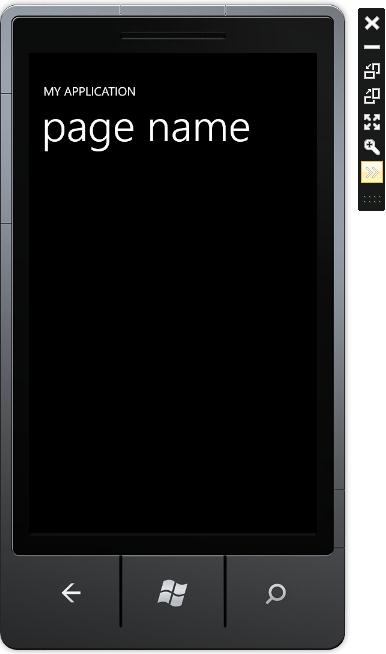
\includegraphics[scale=0.6]{images/emulateur.jpg}
\caption{\'Emulateur Windows Phone}
\end{figure}

\paragraph{}
L'émulateur est muni des trois boutons physiques requis par Microsoft : retour, démarrer, recherche mais aussi d'une barre d'outils. Cette barre est composée des contrôles suivants: 
\begin{itemize}
	\item[•]\textbf{Fermer} : mettre fin à l'émulateur
	\item[•]\textbf{Réduire} : réduit l'émulateur dans la barre de tâches
	\item[•]\textbf{Faire pivoter vers la gauche} ! fait pivoter l'émulateur de 90 degrés dans le sens anti-horaire
	\item[•]\textbf{Faire pivoter vers la droite} : fait pivoter l'émulateur de 90 degrés dans le sens horaire
	\item[•]\textbf{Redimensionner} : redimensionne l'affichage du Windows Phone
	\item[•]\textbf{Zoom} : permet de redimensionner l'émulateur
	\item[•]\textbf{Outils supplémentaires} : accès à l'accéléromètre, gestion de l'emplacement géographique et prise des captures d'écrans
\end{itemize}


	\section{Visual Studio}

	\subsection{Interface de développement}	
\paragraph{}
Visual Studio est l'environnement de développement commun aux deux types de développements supportés parla plateforme mobile : Silverlight et XNA.  

	\begin{figure}[H]
		\center
		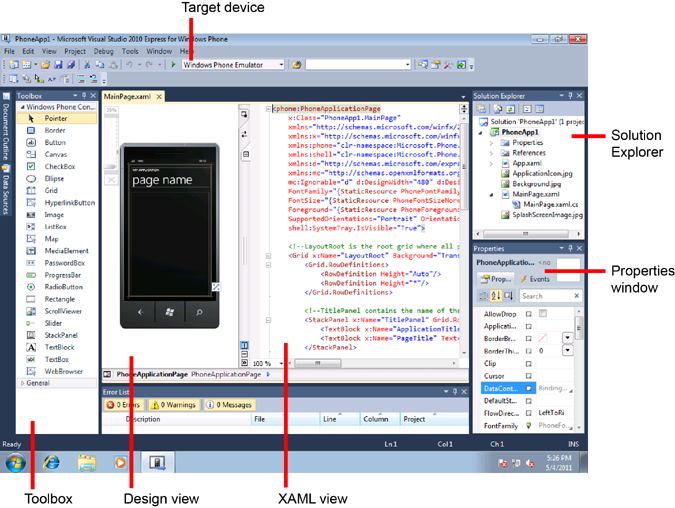
\includegraphics[scale=0.6]{images/visualstudioview.png}
		\caption{Visual Studio 2010 Express pour Windows Phone}
	\end{figure}

\paragraph{}
L'environnement est séparé en différentes parties. La partie centrale et principale est dédiée au code et à la vue du Windows Phone. Sur la gauche se trouve la toolbox répertoriant différents contrôles, et sur la droite, en haut se situe l'explorateur de la Solution\footnote{Dans Visual Studio, un projet est appelé Solution} et en bas la fenêtre de propriétés des contrôles qui sont insérés via la toolbox. 

		\subsection{Création de projet}
%description des différents modèles de projets disponibles
\paragraph{}
Lors de la création d'un projet, Visual Studio propose un ensemble de modèles pour visual Basic et Visual C$\#$ qui sont déclinés pour Silverlight et XNA.

	\begin{figure}[H]
		\center
		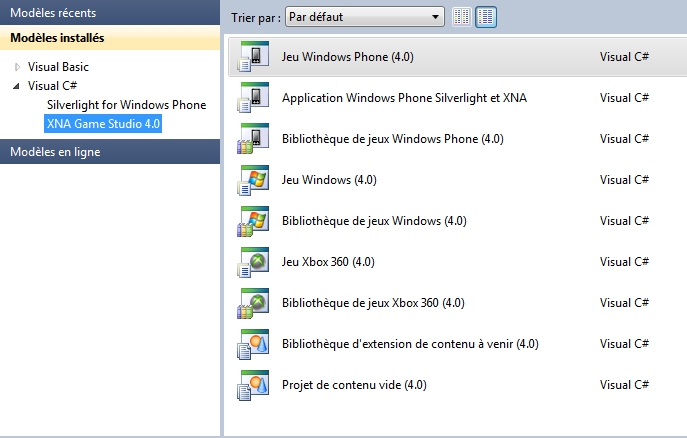
\includegraphics[scale=0.6]{images/creaprojetxna.png}
		\caption{Création de projet avec XNA}
	\end{figure}		

\paragraph{}
Visual Studio propose deux modèles pour XNA : 
\begin{itemize}
	\item[•]\textbf{Jeu Windows Phone (4.0)} : modèle de base pour créer un jeu
	\item[•]\textbf{Bibliothèque de jeu Windows Phone (4.0)} : permet de rajouter des composantes à son application XNA
\end{itemize}
	
	\begin{figure}[H]	
		\center
		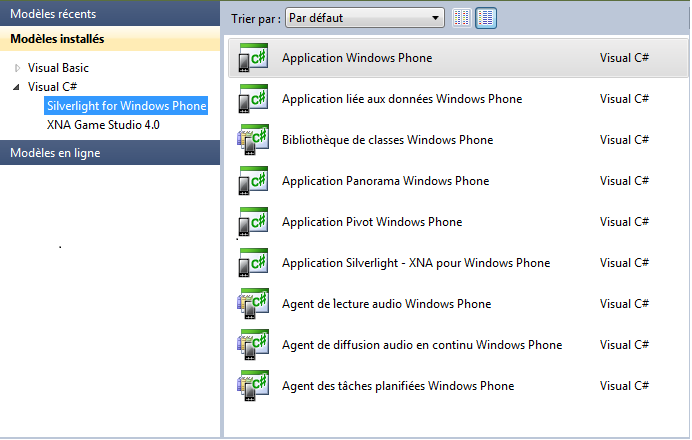
\includegraphics[scale=0.6]{images/creaprojetsilverlight.png}		
		\caption{Création de projet avec Silverlight}
	\end{figure}

\paragraph{}
Pour Silverlight, il propose cinq modèles de projet : 
\begin{itemize}
	\item[•]\textbf{Application Windows Phone} : modèle de base pour commencer d'une page vierge
	\item[•]\textbf{Application liée aux données Windows Phone} : modèle exemple qui contient une ListBox alimentée en données, permet également de voir comment naviguer entre des pages de l'application en cliquant sur un élément de la ListBox
	\item[•]\textbf{Bibliothèque de classes Windows Phone} : projet utiliser pour rajouter des composantes (nouvelles bibliothèque de contrôles, nouveaux modules, classes, etc)
	\item[•]\textbf{Application Panorama Windows Phone} : modèle qui permet de faciliter l'affichage d'un écran trop grand, scinde l'écran en sous-zones et propose une navigation fluide comme si l'on tournait les pages d'un livre
	\item[•]\textbf{Application Pivot Windows Phone} : modèle assez similaire au panorama, mais plus utilisé pour montrer plusieurs pages de la même donnée autour d'un pivot alors que le contrôle Panorama sera plus utilisé pour naviguer entre plusieurs pages
\end{itemize}

		\subsection{Configuration de base}
%description des fichiers générés lors de la création d'un projet		
\paragraph{}
Lors de la création d'un projet à partit d'un modèle une configuration de base est générée pour le projet. Que ce soit Silverlight ou XNA, la structure du projet contient obligatoirement les éléments suivants dans le dossier Propriétés: 
\begin{itemize}
	\item[•]\textbf{AppManifest.xml} : prépare le livrable finale (.xap) en référençant les pré-requis nécessaires à son fonctionnement (les librairies par exemple)
	\item[•]\textbf{WMAppManifest.xml} : fichier de configuration (spécifique à Windows Phone) pour décrire l'applications au travers d'attributs XML (titre, description, nom de l'auteur, société, version, technologie), permet d'identifier l'application après son déploiement
\end{itemize}

\paragraph{}
Certaines images sont aussi générées lors de la création du projet. Cependant leur nom diffère en Silverlight et XNA : 
\begin{itemize}
	\item[•]\textbf{GameThumbnail.png}(XNA)/\textbf{ApplicationIcon.png}(Silverlight) : icône de l'application telle qu'elle sera affichée dans la liste des applications installées sur le téléphone et sur le Marketplace
	\item[•]\textbf{Background.png} : icône de la version "épinglée" de l'application lorque l'utilisateur rajoute l'application dans ses favoris sur la page d'accueil
	\textbf{Game.ico} (XNA) : icône du jeu XNA au format icône Windows pour les jeux compatibles avec Windows
	\item[•]\textbf{SplashScreenImage.jpg} (Silverlight) : image affichée pendant le lancement de l'application 
\end{itemize}

	\begin{figure}[H]	
		\center
		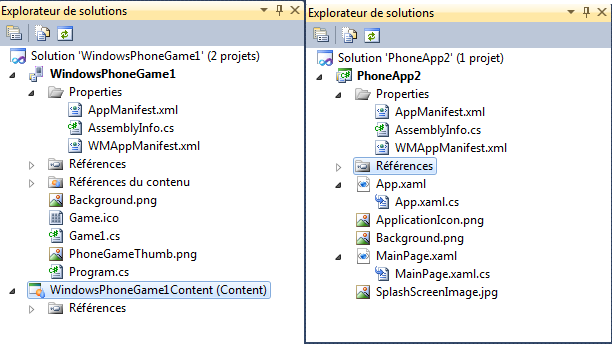
\includegraphics[scale=0.8]{images/explorateursolution.png}		
		\caption{Explorateur de solutions XNA et Silverlight}
	\end{figure}

\paragraph{}
Dans le cas d'une application Silverlight, \textbf{App.xaml} est un fichier qui fait référence aux ressources et qui gère les évènements au niveau de l'application et \textbf{MainPage.xaml}  est le fichier pour gérer le design de la page d'accueil de l'application  avec à gauche la vue du Windows Phone et à droite le code.

	\section{Expression Blend}
	
\paragraph{}
Expression Blend est le logiciel utilisé par les designers de conception graphique. Il n'est utilisé que dans le cadre d'applications Silverlight. Il est possible de créer un nouveau projet à partir d'Expression Blend de développement Windows Phone 7. Mais il est aussi possible de lancer Expression Blend à partir de Visual Studio.

\paragraph{}
Comme pour Visual Studio, avec Expression Blend il est possible d'éditer directement le code en XAML mais le travail est majoritairement réalisé de manière graphique. Le concepteur d'interface dispose d'une palette d'objets graphiques destinés à être simplement glissés-déposés dans la page en édition. Chaque contrôle, une fois positionné, peut être configuré grâce à la fenêtre de propriétés. Le designer peut personnaliser l'objet au niveau des couleurs, dégradé, épaisseur des traits, contenu, style de la police, etc ...
	
	\begin{figure}[H]	
		\center
		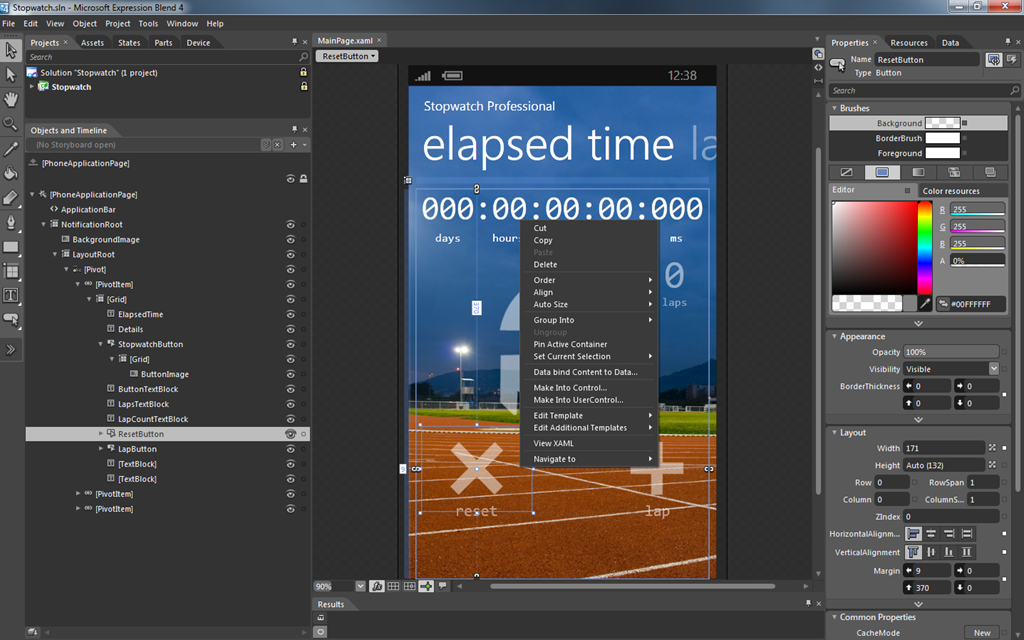
\includegraphics[scale=0.5]{images/expressionblend.png}		
		\caption{Expression Blend 4}
	\end{figure}

	\section{Test sur le matériel}
%comment tester son application sur son telephone, declaration avec Zune
\paragraph{}
Pour tester son application, chaque développeur disposant d'un compte App Hub peut sur un nombre limité d'appareil déployer son application. Car celui-ci ne peut pas passer par le Marketplace pour l'installer et que toute diffusion d'applications s'effectue par le Marketplace. 

\paragraph{}
Un téléphone servant aux tests, doit au préalable avoir été synchronisé avec Zune\footnote{\url{www.zune.net}} qui sert d'interface logicielle entre l'ordinateur et le téléphone. Après la reconnaissance du téléphone par Zune, il faut l'enregistrer. Cela ne peut être fait que par un développeur possédant un compte App Hub valide. Un téléphone ne peut appartenir qu'à un seul compte valide à la fois. L'enregistrement s'efectue au travers d'un outil fournit lors de l'installation de l'environnement de développement : Windows Phone Developper Registration. Le téléphone est ensuite déverrouillé  pour le développement. Il est donc possible de déployer des applications dessus. Il est possible lorsque le téléphone est connecté de tester directement dessus à la place de l'émulateur en choisissant à la place de "Windows Phone 7 Emulator" "Windows Phone 7 Device". Cela permet donc de débugguer depuis son Windows Phone.

%%%%%%%%%%% CHAPITRE SILVERLIGHT %%%%%%%%%%%%%%%%%%%%%

\chapter{Silverlight}

%definitions et explications de ce qu'est le framework silverlight
\paragraph{}
Silverlight est le framework utilisé lors de conception d'application Windows Phone. 

	
	%\section{Différentes classes}
	
	\section{Contrôles de positionnement}
		\subsection{La grille}
\paragraph{}
Le contrôle \textbf{Grid} permet d'organiser une vue en ligne et en colonne. C'est l'équivalent d'un tableau en HTML. Grâce à ce tableau; il sera plus facile de positionner d'autres contrôles. par défaut, une grille ne possède qu'une seule ligne et colonne. 

\begin{lstlisting}[caption={Exemple d'utilisation du contrôle \textbf{Grid}}]
<Grid>
    <Grid.RowDefinitions>
        <RowDefinition Height="*" />
        <RowDefinition Height="*" />
        <RowDefinition Height="*" />
    </Grid.RowDefinitions>
    <Grid.ColumnDefinitions>
        <ColumnDefinition Width="*" />
        <ColumnDefinition Width="*" />
        <ColumnDefinition Width="*" />
    </Grid.ColumnDefinitions>
	<TextBlock Text="O" FontSize="50" Grid.Row="0" Grid.Column="0" HorizontalAlignment="Center" VerticalAlignment="Center" />
    <TextBlock Text="O" FontSize="50" Grid.Row="0" Grid.Column="1" HorizontalAlignment="Center" VerticalAlignment="Center" />
    <TextBlock Text="O" FontSize="50" Grid.Row="0" Grid.Column="2" HorizontalAlignment="Center" VerticalAlignment="Center" />
    <TextBlock Text="X" FontSize="50" Grid.Row="1" Grid.Column="0" HorizontalAlignment="Center" VerticalAlignment="Center" />
    <TextBlock Text="O" FontSize="50" Grid.Row="1" Grid.Column="1" HorizontalAlignment="Center" VerticalAlignment="Center" />
    <TextBlock Text="X" FontSize="50" Grid.Row="1" Grid.Column="2" HorizontalAlignment="Center" VerticalAlignment="Center" />
    <TextBlock Text="O" FontSize="50" Grid.Row="2" Grid.Column="0" HorizontalAlignment="Center" VerticalAlignment="Center" />
    <TextBlock Text="X" FontSize="50" Grid.Row="2" Grid.Column="1" HorizontalAlignment="Center" VerticalAlignment="Center" />
    <TextBlock Text="X" FontSize="50" Grid.Row="2" Grid.Column="2" HorizontalAlignment="Center" VerticalAlignment="Center" />
</Grid>
\end{lstlisting}

Dans cet exemple, tout d'abord une grille de trois lignes et colonnes sont définies. Ensuite sont crée neuf zone de texte contenant soit "X" soit "O". Leur contenu sera centré horizontalement et verticalement et aura une taille de 50. A chaque zone de texte, o, lui indique sur quelle ligne et colonne elle doit se placer. Ce qui donne le rendu suivant : 
\begin{figure}[H]
	\center
	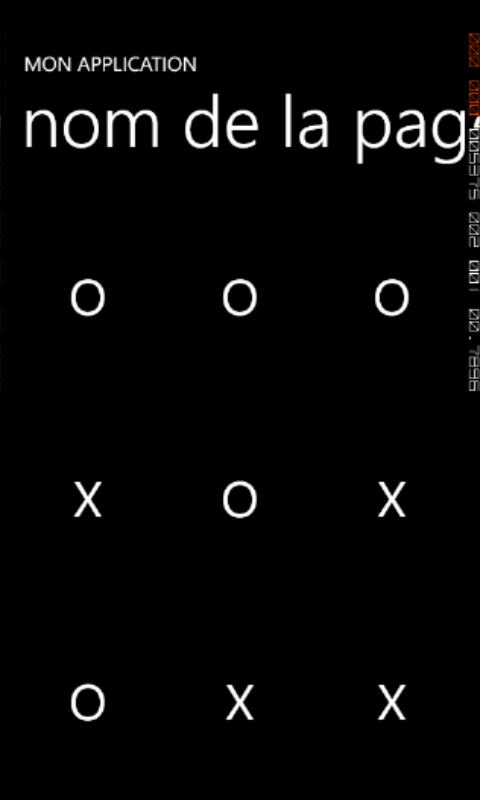
\includegraphics[scale=0.3]{images/morpion.png}
	\caption{Grille 3x3}
\end{figure}

		
		\subsection{Le stackpanel}
		
\paragraph{}
Le contrôle \textbf{StackPanel} permet d’empiler les contrôles les uns à la suite des
autres verticalement ou horizontalement. 

\begin{lstlisting}[caption={Exemple d'utilisation du contrôle \textbf{StackPanel}}]
	<StackPanel>
		<Button Content="Button1" Height="71" Name="button1" Width="447" />
		<Button Content="Button2" Height="71" Name="button2" Width="447" />
		<Button Content="Button3" Height="71" Name="button3" Width="447" />
	</StackPanel>
\end{lstlisting}
	
\paragraph{}
Le code ci-dessus donnera l'exemple suivant : 

\begin{figure}[H]
	\center
	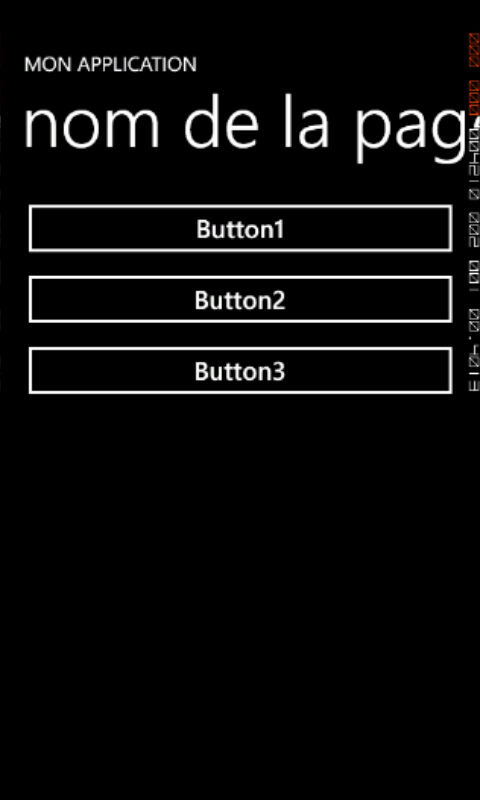
\includegraphics[scale=0.3]{images/stackpanel.png}
	\caption{Empilement vertical de bouton avec le StackPanel}
\end{figure}	
		
		\subsection{Le canvas}

\paragraph{}
Le contrôle \textbf{Canvas} permet de placer les éléments de façon absolue par coordonnées. L'origine du canvas (le point (0,0)) se situe dans le coin supérieur gauche du contrôle. 

\begin{lstlisting}[caption={Exemple d'utilisation du contrôle \textbf{Canvas}}]
    <Canvas>
        <TextBlock Text="Je suis en bas a gauche" Canvas.Top="500" />
        <TextBlock Text="Je suis en haut a droite" Canvas.Left="250" Canvas.Top="10"/>
    </Canvas>
\end{lstlisting}

\paragraph{}
Dans cet exemple, un canvas contenant deux zones de texte est défini. Les zones de texte sont placés dans le canvas à l'aide des attributs \textbf{Canvas.top} (coordonnée sur l'axe des Y) et \textbf{Canvas.Left} (coordonée sur l'axe des X). Cet exemple de canvas donnera le résultat suivant : 

\begin{figure}[H]
	\center
	
\includegraphics[scale=0.3]{images/canvas.png}
	\caption{Affichage du texte avec un \textbf{Canvas}}
\end{figure}

	\section{Contrôles d'entrée utilisateur}
		\subsection{TextBox}
		
\paragraph{}
Le contrôle \textbf{TextBox} permet à l'utilisateur de saisir du texte. Il est possible de préciser une valeur par défaut au  contrôle en remplissant le champ \textbf{Text}. L'exemple ci-dessous générera une une zone de texte pré-remplie avec la valeur "Prenom" que l'utilisateur pourra modifier.

\begin{lstlisting}[caption={Exemple d'utilisation du contrôle \textbf{TextBox}}]
    <TextBox x:Name="nom" Text="Prenom" />
\end{lstlisting}

\paragraph{}
Il est possible de récupérer le texte saisit par l'utilisateur avec la propriété \textbf{Text} du contrôle. Pour cela, il faut déclarer une variable qui prendra la valeur saisie.

\begin{lstlisting}[caption={Récupération du texte saisit}]
	string prenom = nom.Text;
\end{lstlisting}
		
		\subsection{CheckBox et RadioButton}

\paragraph{}
Les contrôles \textbf{CheckBox} et \textbf{RadioButton} permettent à l'utilisateur d'effectuer un choix parmi une liste d'options. Le RadioButton, contrairement au CheckBox ne permet de ne choisir qu'une unique option dans une liste. 

\begin{lstlisting}[caption={Exemple d'utilisation du contrôle \textbf{CheckBox} et \textbf{RadioButton}}]
    <CheckBox x:Name="caseACocher" Checked="case_ Checked" Unchecked ="case_Unchecked"/>
    <RadioButton x:Name="boutonACocher" />
\end{lstlisting}

\paragraph{}
Il est possible de récupérer l'état d'un CheckBox et d'un RadioButton avec la boucle if suivante : 

\begin{lstlisting}[caption={Récupération de l'état d'un \textbf{CheckBox} et d'un \textbf{RadioButton}}]
	if(caseACocher.IsChecked){ \\ou (boutonACocher.IsChecked)
		\\ traitement
	]else{
		\\traitement
	}
\end{lstlisting}

\paragraph{}
Ces deux contrôles possèdent deux évènements : \textbf{Checked} et \textbf{Unchecked}. Ce qui permet de réaliser une action si une case est cochée et de réaliser un traitement lorsque bouton radio est coché.
 
\begin{lstlisting}[caption={Gestionnaire d'événements du contrôle \textbf{CheckBox}}]
	private void case_ Checked(object sender, EventArgs e){
		\\ traitement quand la case est coche
	}
	private void case_ Unchecked(object sender, EventArgs e){
		\\ traitement quand la case est decoche
	}
	
\end{lstlisting}
		
	\section{Autres contrôles}
		\subsection{Button}
		
\paragraph{}
Le contrôle \textbf{Button} permet d'ajouter un bouton. L'attribut \textbf{Content} permet de définir le texte afficher dans le bouton.

\begin{lstlisting}[caption={Gestionnaire d'événements du contrôle \textbf{CheckBox}}]
	<Button x:Name="bouton" Content="Cliquez" Click="bouton_click />	
\end{lstlisting}

Lorsque l'utilisateur clique dessus, il peut déclencher une action. Cela est réalisé par l'attribut \textbf{Click}.

\begin{lstlisting}[caption={Gestionnaire d'événements du contrôle \textbf{Button}}]
	private void bouton_click(object sender, RoutedEventArgs e){
		\\ traitement quand on clique sur le bouton
	}
	
\end{lstlisting}

		\subsection{ScrollViewer}

\paragraph{}
Le contrôle \textbf{ScrollViewer} permet d'afficher un élément dans une zone plus petite que sa taille réelle grâce à la barre de défilement.
 
\begin{lstlisting}[caption={Exemple d'utilisation du contrôle \textbf{ScrollViewer}}]
<ScrollViewer>
    <StackPanel>
        <TextBlock Text="Bonjour a tous 1" Margin="40" />
        <TextBlock Text="Bonjour a tous 2" Margin="40" />
        <TextBlock Text="Bonjour a tous 3" Margin="40" />
        <TextBlock Text="Bonjour a tous 4" Margin="40" />
        <TextBlock Text="Bonjour a tous 5" Margin="40" />
        <TextBlock Text="Bonjour a tous 6" Margin="40" />
        <TextBlock Text="Bonjour a tous 7" Margin="40" />
        <TextBlock Text="Bonjour a tous 8" Margin="40" />
        <TextBlock Text="Bonjour a tous 9" Margin="40" />
        <TextBlock Text="Bonjour a tous 10" Margin="40" />
    </StackPanel>
</ScrollViewer>
\end{lstlisting}
	
\paragraph{}	
Toutes les zones de textes n'apparaissent pas à l'écran avec l'exemple précédent, l'utilisateur devra donc faire défiler le texte pour voir les dernières zones.

\begin{figure}[H]
	\center
	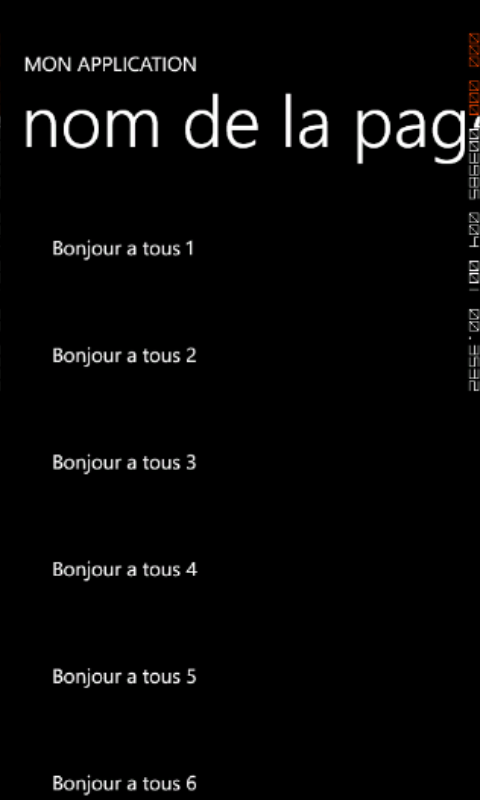
\includegraphics[scale=0.3]{images/scrollviewer.png}
	\caption{Affichage du texte avec \textbf{ScrollViewer}}
\end{figure}
		
	\section{Manipulation des images}
	
\paragraph{}
Pour afficher une image dans l'application, il faut utiliser le contrôle \textbf{Image}.

\begin{lstlisting}[caption={Exemple d'utilisation du contrôle \textbf{Image}}]
	<Image x:Name="logo" Source="images/monimage.png" />	
\end{lstlisting}	

Avant de renseigner le contrôle Image, l'image que l'on veut afficher doit être embarquer dans le projet. Pour cela en faisant un clic droit dans l'explorateur de la solution, on sélectionnera tout d'abord le menu \textbf{ajouter} puis \textbf{ajouter un élément existant}.

	\section{Geolocalisation}
		\subsection{Geolocalisation du smartphone}

\paragraph{}
La position géographique du téléphone peut être déterminé grâce à la classe \textbf{GeoCoordinateWatcher}. Pour pouvoir l'utiliser, il faut faire une référence à l'assemblage \textbf{System.Device.dll} et ajouter l'espace de nom \textbf{System.Device.Location}. La position sera récupérée avec l'évènement \textbf{PositionChanged}. Pour démarrer le GPS, il faut appeler la méthode \textbf{start()}.

\begin{lstlisting}[caption={Affichage des coordonnées du téléphone}]
// Code dans MainPage.xaml.cs
using System.Device.Location;

namespace PhoneApp2
{
    public partial class MainPage : PhoneApplicationPage
    {
        // Constructeur
        public MainPage()
        {
            InitializeComponent();
            var geoWatcher = new GeoCoordinateWatcher();

            geoWatcher.PositionChanged += (s, e) =>
               {
            latitude.Text = e.Position.Location.Latitude.ToString();
            longitude.Text = e.Position.Location.Longitude.ToString();
               };
            geoWatcher.Start();
        }
    }
}

// Code dans MainPage.xaml
<StackPanel>    
	<TextBlock Height="30"  Name="latitude" Text="TextBlock"  />
    <TextBlock Height="30"  Name="longitude" Text="TextBlock"  />
</StackPanel> 

\end{lstlisting}	

\paragraph{}	
On peut modifier la position géographique de l'émulateur avec l'outil \textbf{Emplacement}. 

\begin{figure}[H]
	\center
	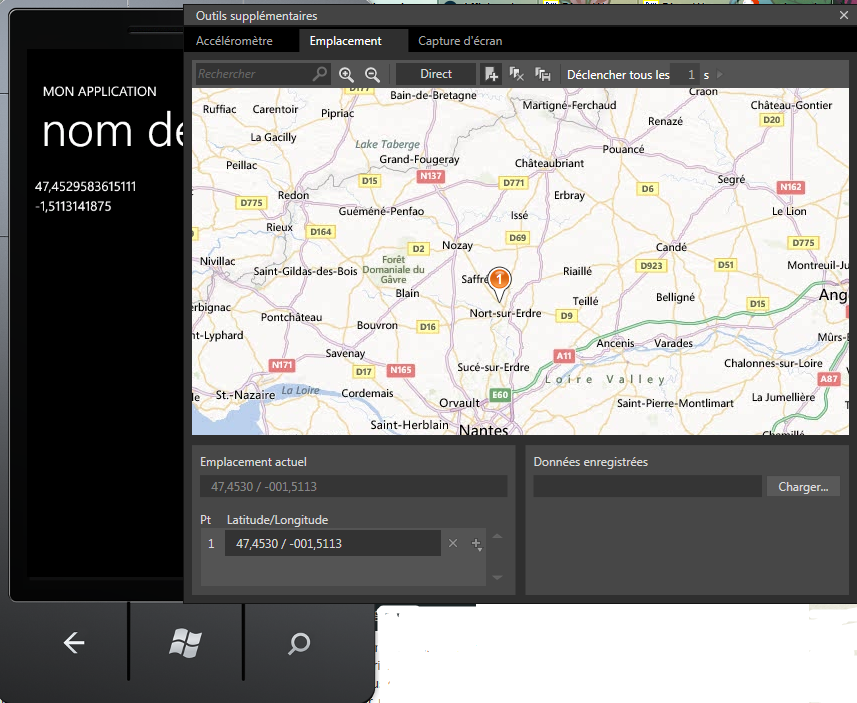
\includegraphics[scale=0.7]{images/geolocalisation.png}
	\caption{Modification de la position de l'émulateur}
\end{figure}
	
	
		\subsection{Bing Maps}
		
\paragraph{}
La représentation géographique d'une position est possible avec le contrôle \textbf{Bing Maps} de classe \textbf{Map}. Pour utiliser cette classe, il faut ajouter l'espace nom et faire référence à l'assemblage \textbf{Microsoft.Phone.Control.Maps}. Il est nécessaire de s'enregistrer sur le site \url{www.bingmapsportal.com} pour utiliser les cartes de Bing. Après l'inscription, qui est gratuite, une clé est obtenue. Elle est à insérer dans le code XAML. 

\begin{lstlisting}[caption={Utilisation de la carte avec le contrôle \textbf{Bing Maps}}]
// ajout de l'espace nom du controle
xmlns:carte="clr-namespace:Microsoft.Phone.Controls.Maps;assembly=Microsoft.Phone.Controls.Maps"	
	
// ajout de la carte	
	<carte:Map x:Name="map" ZoomBarVisibility="Visible"/>
\end{lstlisting}

\paragraph{}
L'attribut \textbf{ZoomBarVisibility} permet d'afficher les contrôles du zoom.

\begin{figure}[H]
	\center
	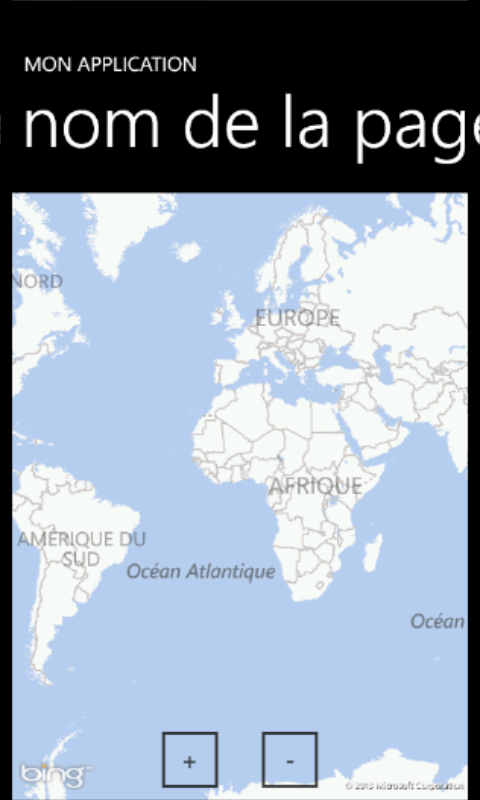
\includegraphics[scale=0.4]{images/bing.png}
	\caption{Affichage de la carte avec les contrôles du zoom}
\end{figure}

	\section{Orientation de l'application}

\paragraph{}
Le téléphone est orientable soit en mode portrait soit en mode paysage. Le développeur peut choisir si son application sera compatible avec une ou les deux orientations et quelle sera l'orientation au démarrage avec les propriétés \textbf{SupportedOrientations} et \textbf{Orientation}.

\begin{lstlisting}[caption={Orientation du téléphone}]
<phone:PhoneApplicationPage 
	SupportedOrientations="PortraitOrLandscape" Orientation="Portrait"
\end{lstlisting}

\paragraph{}
Avec code ci-dessus, l'application s'ouvrira en mode Portrait mais supportera le mode paysage. Les propriétés SupportedOrientations et Orientation peuvent prendre les valeurs suivantes : 
\begin{itemize}
	\item[•] Portrait
	\item[•] Landscape
	\item[•] PortaitOrLandscape
\end{itemize}
	
		
%%%%%%%%%%%% CHAPITRE 4 LECTEUR RSS %%%%%%%%%%%%%%%%%%%%%%

\chapter{Lecteur RSS}
	\section{Flux RSS et applications}
		\subsection{Flux RSS}
%defintion d'un flux rss
		
		\subsection{Applications existantes}
%présentation des applis déja existante sur le markerplace

	\section{Lecteur RSS}
	
%Explication sur notre appli : comment ca fonctionne, comment la faire .... 

%%%%%%%%%%%%% CONCLUSION %%%%%%%%%%%%%%%%%%%%

\chapter{Conclusion}

%\annexes

\addcontentsline{toc}{chapter}{\numberline{}Index}
\printindex

\end{document}

